% Uncomment for flat handout (no overlay duplicates):
%\documentclass[aspectratio=169,10pt,handout]{beamer}
\documentclass[aspectratio=169,10pt]{beamer}

\usetheme{metropolis}
\usepackage{appendixnumberbeamer}
\usepackage{booktabs}
\usepackage{amsmath,amssymb}
\usepackage{tikz}
\usetikzlibrary{arrows.meta,positioning,calc,decorations.pathreplacing,shapes.geometric,fit}
\usepackage{pgfplots}
\pgfplotsset{compat=1.18}
\usepackage{xcolor}
\usepackage{multicol}
\usepackage{graphicx}
\usepackage{hyperref}
\hypersetup{colorlinks=true,urlcolor=columbia,linkcolor=columbia}

\definecolor{columbia}{RGB}{29,79,145}
\definecolor{columbialight}{RGB}{117,170,219}
\definecolor{columbiaaccent}{RGB}{210,73,42}
\definecolor{columbiagray}{RGB}{117,117,117}
\definecolor{softbg}{RGB}{245,245,250}
\definecolor{hlgreen}{RGB}{46,139,87}

\setbeamercolor{frametitle}{bg=columbia,fg=white}
\setbeamercolor{progress bar}{fg=columbiaaccent}
\setbeamercolor{alerted text}{fg=columbiaaccent}
\setbeamercolor{block title}{bg=columbia,fg=white}
\setbeamercolor{block body}{bg=softbg}
\setbeamerfont{title}{size=\Large,series=\bfseries}
\setbeamerfont{subtitle}{size=\normalsize}

\graphicspath{{./figures/}}

\title{Lecture 23: Population Health Data \& Survival Analysis}
\subtitle{BINF 4002 --- Machine Learning for Health}
\author{Matthew McDermott}
\institute{Dept.\ of Biomedical Informatics, Columbia University}
\date{April 14, 2026}

\begin{document}

\begin{frame}[noframenumbering]
\maketitle
\end{frame}

% ============================================================
\begin{frame}{Where We Are}
\textbf{Modality progression:}
\begin{itemize}
    \item[\textcolor{columbiagray}{$\bullet$}] L17--18: EHR \& Claims \quad
          \textcolor{columbiagray}{$\bullet$} L19--20: Clinical Text \& NLP \quad
          \textcolor{columbiagray}{$\bullet$} L21--22: Clinical Imaging
    \item[\textcolor{columbiaaccent}{$\to$}] \alert{L23: Population Health Data \& Survival Analysis} $\gets$ \textbf{today}
    \item[\textcolor{columbiagray}{$\circ$}] L24: Causality \& Fairness \quad L25+: Omics, Molecules, Deployment
\end{itemize}

\vspace{0.3em}
\textbf{Today has two parts:}
\begin{enumerate}
    \item \textbf{Population health data:} registries, biobanks, and clinical trials---\emph{designed} data, in contrast to the \emph{byproduct} data of L17--22.
    \item \textbf{Survival analysis:} a modeling technique for time-to-event outcomes, common in this domain and many others.
\end{enumerate}
\end{frame}

% ============================================================
\section{Part I: Population Health Data}
% ============================================================

% --- Point 1: separate attempt from problem ---
\begin{frame}{A Question}
\textbf{Which treatment for kidney stones is better---open surgery (A) or percutaneous nephrolithotomy (B)?}

\vspace{0.3em}
\textbf{Attempt 1: Use the EHR.}

You have your hospital's data. Some patients received Treatment A, some B. You could compare their success rates.

\vspace{0.3em}
\textit{What could go wrong?}
\end{frame}

% --- Point 1: problems on separate slide, no blank first overlay ---
\begin{frame}{Why the EHR Isn't Enough}
\textbf{Several problems:}
\begin{itemize}[<+->]
    \item \textbf{One health system.} Specific patient population, geographic bias---not representative.
    \item \textbf{Small numbers.} Concentrated in a narrow time window---underpowered.
    \item \textbf{Severity not well-captured.} Patients may only present when stones are severe; mild cases go elsewhere or self-resolve.
    \item \textbf{Treatment choice reflects clinician judgment.} Surgeons pick the procedure based on the case---selection bias by indication.
\end{itemize}

\onslide<5->{
\vspace{0.2em}
\textbf{So EHR data alone won't give us a reliable answer. What else could we try?}}
\end{frame}

% --- Points 2, 3: hospitals or individuals; Treatment A first ---
\begin{frame}{Attempt 2: Registry Data}
\textbf{Suppose we survey many hospitals and individuals.} Collect data on everyone who had Treatment A or B, their outcomes, and key patient characteristics. This is \textbf{registry data}---designed to capture a broad population.

\vspace{0.3em}
Better geographic coverage, more patients, standardized data collection.

\vspace{0.3em}
\pause
\textbf{The result:}
\begin{center}
{\small Treatment A (open surgery): 78\% success. \quad Treatment B (PCNL): 83\% success.}
\end{center}

\vspace{0.1em}
Treatment B looks better. Done?
\end{frame}

% --- Points 4: drop L8/L24 line ---
\begin{frame}{Not So Fast: Simpson's Paradox}
\textbf{Kidney stone treatment data} (Charig et al., 1986):

\vspace{0.1em}
\begin{center}
{\small
\renewcommand{\arraystretch}{1.15}
\only<1>{%
\begin{tabular}{lccc}
\toprule
& \textbf{Open surgery (A)} & \textbf{PCNL (B)} & \textbf{``Better''} \\
\midrule
\textbf{Overall} & 78\% success & 83\% success & B \\
\bottomrule
\end{tabular}
}%
\only<2>{%
\begin{tabular}{lccc}
\toprule
& \textbf{Open surgery (A)} & \textbf{PCNL (B)} & \textbf{``Better''} \\
\midrule
\textbf{Overall} & 78\% success & 83\% success & B \\
\midrule
Small stones & 93\% & 87\% & A \\
\bottomrule
\end{tabular}
}%
\only<3->{%
\begin{tabular}{lccc}
\toprule
& \textbf{Open surgery (A)} & \textbf{PCNL (B)} & \textbf{``Better''} \\
\midrule
\textbf{Overall} & 78\% success & 83\% success & B \\
\midrule
Small stones & 93\% & 87\% & A \\
Large stones & 73\% & 69\% & A \\
\bottomrule
\end{tabular}
}%
}
\end{center}

\only<4->{
\vspace{0.1em}
A is better in \emph{every subgroup}, but worse overall. Open surgery was assigned to large (harder) stones---confounding by severity.

\vspace{0.1em}
\begin{center}
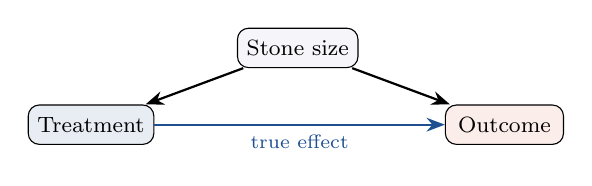
\begin{tikzpicture}[
    box/.style={draw,rounded corners,minimum width=1.5cm,minimum height=0.5cm,align=center,font=\footnotesize,fill=softbg},
    >=Stealth, scale=0.75
]
\node[box] (conf) at (3.5,1.3) {Stone size};
\node[box,fill=columbia!10] (treat) at (0,0) {Treatment};
\node[box,fill=columbiaaccent!10] (out) at (7,0) {Outcome};
\draw[->,thick] (conf) -- (treat);
\draw[->,thick] (conf) -- (out);
\draw[->,thick,columbia] (treat) -- (out) node[midway,below,font=\scriptsize] {true effect};
\end{tikzpicture}
\end{center}
}
\end{frame}

% ============================================================
\begin{frame}{Simpson's Paradox in Real Health Data}
\begin{center}
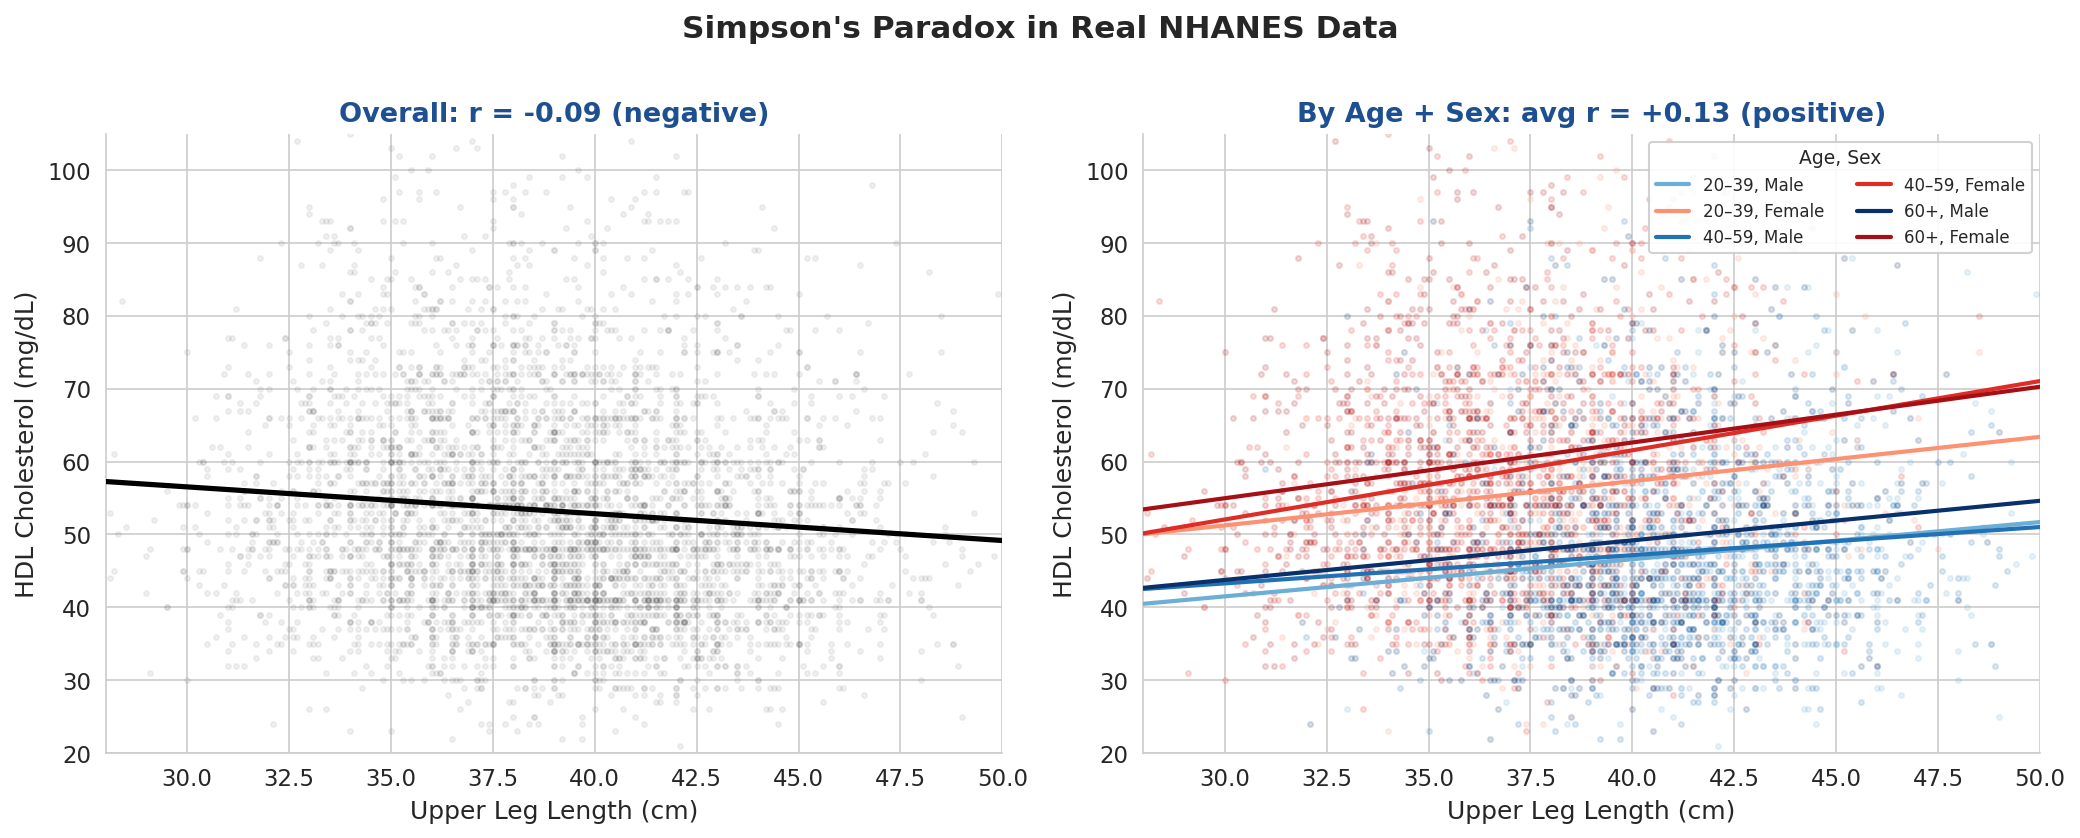
\includegraphics[width=\textwidth,height=0.68\textheight,keepaspectratio]{fig_simpsons_nhanes.png}
\end{center}
\vspace{-0.3em}
{\scriptsize Real NHANES 2017--2018 data. Overall, longer legs correlate with \emph{lower} HDL cholesterol ($r = -0.09$). Within every age+sex subgroup, the relationship reverses ($\text{avg } r = +0.13$). Men have longer legs \emph{and} lower HDL---aggregating across sex and age reverses the within-group trend.}
\end{frame}

% ============================================================
\begin{frame}{What Registries Can and Can't Tell You}
\textbf{Registries are good at:}
\begin{itemize}
    \item Describing \emph{what happened}---incidence, outcomes, trends
    \item Broad coverage across populations and geographies
    \item Generating hypotheses about treatment effects
\end{itemize}

\vspace{0.2em}
\pause
\textbf{Registries struggle with:}
\begin{itemize}
    \item Answering \emph{what would have happened under a different treatment}
    \item Confounders must be measured \emph{and} adjusted for---Simpson's Paradox shows what goes wrong when they aren't
\end{itemize}

\vspace{0.2em}
\textbf{For the most reliable causal answer, we'd need randomization.}
\end{frame}

% --- Point 5: Travers et al. citation ---
\begin{frame}{Randomized Trials}
\begin{center}
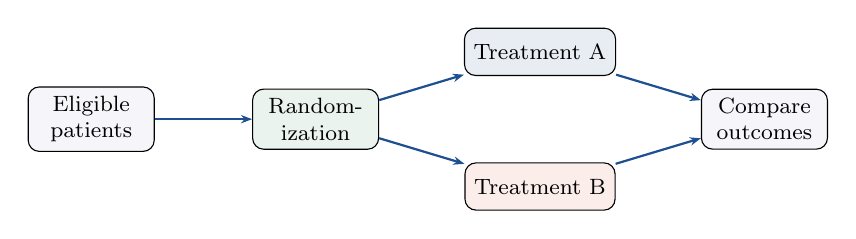
\begin{tikzpicture}[
    box/.style={draw,rounded corners,minimum width=1.6cm,minimum height=0.6cm,align=center,font=\footnotesize,fill=softbg},
    arr/.style={-{Stealth[length=4pt]},thick,columbia}, scale=0.95
]
\node[box] (pop) at (0,0) {Eligible\\patients};
\node[box,fill=hlgreen!10] (rand) at (3,0) {Random-\\ization};
\node[box,fill=columbia!10] (tx) at (6,0.9) {Treatment A};
\node[box,fill=columbiaaccent!10] (ctrl) at (6,-0.9) {Treatment B};
\node[box] (out) at (9,0) {Compare\\outcomes};
\draw[arr] (pop) -- (rand);
\draw[arr] (rand) -- (tx);
\draw[arr] (rand) -- (ctrl);
\draw[arr] (tx) -- (out);
\draw[arr] (ctrl) -- (out);
\end{tikzpicture}
\end{center}

\vspace{0.1em}
\textbf{Randomization} balances confounders---measured \emph{and} unmeasured---in expectation.

\vspace{0.1em}
\pause
\textbf{But:} expensive (\$10K--50K per patient for Phase III), sometimes unethical, and the enrolled population is narrow.

\vspace{0.1em}
{\small
\textbf{How narrow?}
Murthy et al.\ (2004): $<$25\% of cancer trial participants were $>$65, despite $>$60\% of cancer in that age group.
Travers et al.\ (2007): only $\sim$4\% of community asthma patients would have met eligibility for the major RCTs behind their treatment guidelines.}
\end{frame}

% --- Point 6: causal inference lead-in ---
\begin{frame}{The Question Determines the Data}
\begin{center}
{\small
\renewcommand{\arraystretch}{1.2}
\begin{tabular}{lp{3.5cm}p{3cm}p{3cm}}
\toprule
\textbf{Question type} & \textbf{Example} & \textbf{Data source} & \textbf{Key risk} \\
\midrule
Descriptive & What is the 5-year survival rate for this cancer? & Registry, cohort & Selection bias \\
Predictive & Will \emph{this patient} respond to treatment? & Any with outcomes & Distribution shift \\
Causal & Does Treatment A \emph{cause} better outcomes than B? & RCT; or observational with causal methods & Confounding \\
\bottomrule
\end{tabular}
}
\end{center}

\vspace{0.1em}
\pause
\textbf{Causal inference methods} (propensity scores, instrumental variables, etc.)\ can enable causal claims from observational data---including EHR---if done carefully. Example: COVID-19 vaccine effectiveness studies from EHR data. \textbf{Thursday (L24)} formalizes this.
\end{frame}

% ============================================================
\begin{frame}{The Data Spectrum}
\begin{center}
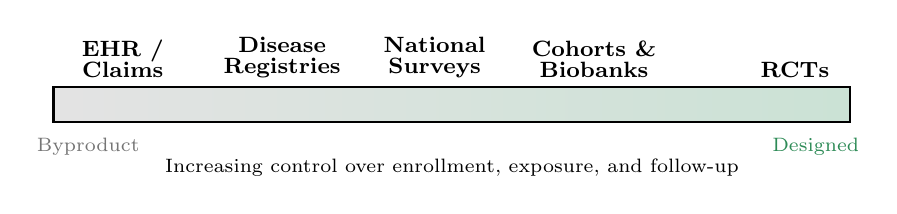
\begin{tikzpicture}[>=Stealth,scale=0.88]
    \shade[left color=columbiagray!20, right color=hlgreen!25]
        (0,0) rectangle (11.5,0.5);
    \draw[thick] (0,0) rectangle (11.5,0.5);

    \node[above,font=\footnotesize\bfseries,align=center] at (1.0,0.5) {EHR /\\[-2pt]Claims};
    \node[above,font=\footnotesize\bfseries,align=center] at (3.3,0.5) {Disease\\[-2pt]Registries};
    \node[above,font=\footnotesize\bfseries,align=center] at (5.5,0.5) {National\\[-2pt]Surveys};
    \node[above,font=\footnotesize\bfseries,align=center] at (7.8,0.5) {Cohorts \&\\[-2pt]Biobanks};
    \node[above,font=\footnotesize\bfseries,align=center] at (10.7,0.5) {RCTs};

    \node[below,font=\scriptsize,columbiagray] at (0.5,-0.1) {Byproduct};
    \node[below,font=\scriptsize,hlgreen] at (11.0,-0.1) {Designed};
    \node[below,font=\scriptsize] at (5.75,-0.4) {Increasing control over enrollment, exposure, and follow-up};
\end{tikzpicture}
\end{center}

\vspace{0.2em}
These are \emph{alternative} data sources, not stages. Modern biobanks blur the boundary.

\vspace{0.2em}
\textbf{Next:} we'll look at specific registries, biobanks, and trial designs in more depth.
\end{frame}

% ============================================================
\section{Data Sources in Depth}
% ============================================================

\subsection{Registries \& Cohorts}

\begin{frame}[standout]
    Registries \& Cohorts
\end{frame}

\begin{frame}{What Does Designed Population Data Look Like?}
\textbf{NHANES} (National Health and Nutrition Examination Survey) is a good example of designed population data:
\begin{itemize}
    \item About 9{,}000 examined participants per 2-year cycle
    \item Home interview (demographics, medical history, diet) + clinic visit (physical exam, labs, questionnaires)
    \item Complex survey design: deliberately oversamples minorities, elderly, low-income
    \item Public data, no credentialing: \href{https://wwwn.cdc.gov/nchs/nhanes/}{\texttt{\small wwwn.cdc.gov/nchs/nhanes/}}
\end{itemize}

\vspace{0.2em}
\pause
\textbf{Key for ML:} Unweighted statistics describe the \emph{sample}; weighted statistics describe the \emph{population}. Missingness is mostly by protocol (``this module wasn't administered this cycle''), not informative---unlike EHR data.

\vspace{0.1em}
{\scriptsize \textbf{Questionnaire PDFs:} \href{https://wwwn.cdc.gov/nchs/nhanes/continuousnhanes/questionnaires.aspx?BeginYear=2017}{\texttt{wwwn.cdc.gov/nchs/nhanes/.../questionnaires.aspx}}}
\end{frame}

% ============================================================
\begin{frame}{NHANES: Variable Structure (Notebook Fig.~1)}
\begin{center}
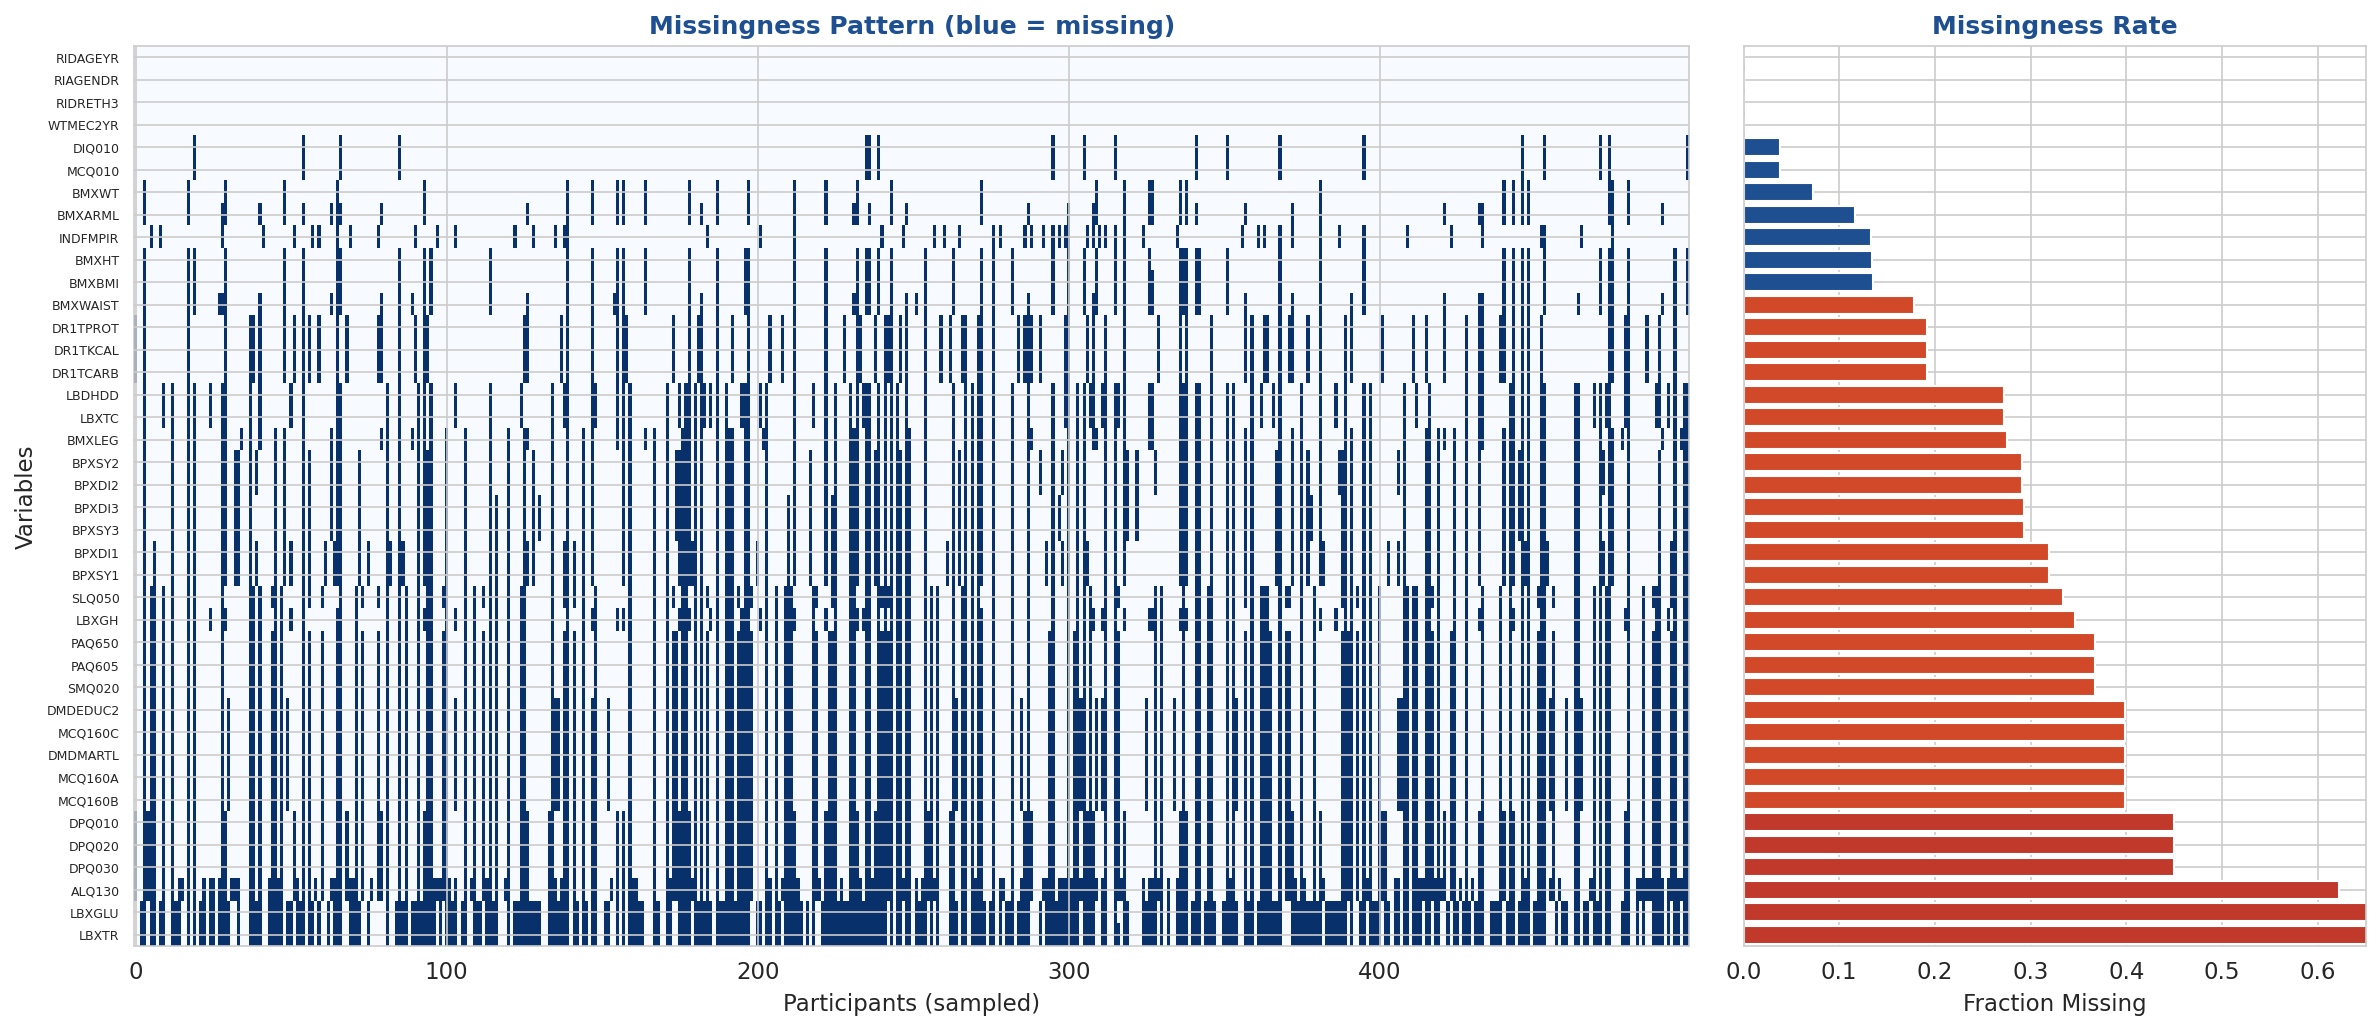
\includegraphics[width=\textwidth,height=0.62\textheight,keepaspectratio]{fig1_nhanes_missingness.png}
\end{center}
\vspace{-0.3em}
{\scriptsize Real NHANES 2017--2018 data (about 9{,}000 participants, about 40 variables, 16 survey components). Left: missingness heatmap---note block structure. Right: per-variable fraction missing. Variable names follow CDC conventions: \textbf{BMXBMI} = Body Mass Index, \textbf{BPXSY1} = Systolic Blood Pressure (1st reading), \textbf{LBXTR} = Triglycerides, \textbf{LBXGLU} = Fasting Glucose, \textbf{DR1TKCAL} = Dietary Recall Calories, \textbf{DPQ010} = Depression Screener (PHQ-9 Q1).}
\end{frame}

% ============================================================
\begin{frame}{SEER: Cancer Surveillance}
\textbf{Surveillance, Epidemiology, and End Results:}
\begin{itemize}
    \item Covers about 46\% of the US population
    \item Cancer incidence, treatment, survival by site, stage, demographics
    \item Research Data: signed agreement; Research Plus: eRA Commons
    \item \href{https://seer.cancer.gov/data/}{\texttt{\small seer.cancer.gov/data/}}
\end{itemize}

\vspace{0.2em}
\pause
\textbf{One lesson from SEER:} large-scale descriptive survival data, but limited confounder control. Treatment assignment is not randomized, so hazard ratios are associational.

\vspace{0.1em}
\textbf{Limitations:} No detailed treatment data, no imaging, limited labs. Geographic selection.
\end{frame}

% ============================================================
\begin{frame}{Biobanks: Designed Cohorts That Blur the Boundary}
\begin{center}
{\small
\renewcommand{\arraystretch}{1.15}
\begin{tabular}{p{2.2cm}rp{2cm}p{4.8cm}}
\toprule
\textbf{Biobank} & \textbf{N} & \textbf{Country} & \textbf{Key features} \\
\midrule
UK Biobank & $\sim$500K & UK & Imaging + genomics + GP/EHR linkage \\
All of Us & $\sim$850K & US & Diversity emphasis, EHR-linked, wearables \\
Japan Biobank & $\sim$270K & Japan & Disease-focused recruitment \\
\bottomrule
\end{tabular}
}
\end{center}

\vspace{0.1em}
\textbf{One lesson from biobanks:} designed enrollment with EHR linkage blurs the byproduct/designed boundary. Participants consented to research, but their clinical data is byproduct.

\vspace{0.1em}
\pause
{\small \href{https://ukbiobank.ac.uk}{\texttt{ukbiobank.ac.uk}} \quad \href{https://allofus.nih.gov}{\texttt{allofus.nih.gov}} \quad \href{https://biobankjp.org}{\texttt{biobankjp.org}}}
\end{frame}

% ============================================================
\begin{frame}{The Healthy Volunteer Effect}
\textbf{People who volunteer for research are systematically different.}

\vspace{0.2em}
\begin{itemize}
    \item Fry et al.\ (2017): UK Biobank participants had \textbf{40--50\% lower all-cause mortality} than the UK average. Response rate: 5.5\%.
    \item Batty et al.\ (2020): despite strong selection into UK Biobank, many risk factor--mortality associations were similar to those in more representative cohorts---but absolute rates and participant composition are biased.
    \item Volunteer-based cohort studies (Framingham, etc.)\ generally enroll healthier, more health-conscious participants than the general population.
\end{itemize}

\vspace{0.2em}
\pause
\textbf{All of Us} deliberately oversamples underrepresented groups---but still faces within-stratum volunteer bias.

\vspace{0.1em}
A model trained on biobank volunteers may not generalize. The bias is in \emph{who enrolls}, not in the measurements.
\end{frame}

% ============================================================
\subsection{Clinical Trials}

\begin{frame}[standout]
    Clinical Trials
\end{frame}

\begin{frame}{RCTs Are Not One Thing}
\begin{center}
{\small
\renewcommand{\arraystretch}{1.15}
\begin{tabular}{p{2.5cm}p{2.8cm}p{3cm}p{2.8cm}}
\toprule
\textbf{Design} & \textbf{What's randomized} & \textbf{Example} & \textbf{When to use} \\
\midrule
Parallel-group & Patients $\to$ arms & Most drug trials & Default design \\
Crossover & Patients $\to$ sequence & Chronic disease & Patient is own control \\
Cluster & Sites / clinics & Implementation science & Group-level intervention \\
Pragmatic & Patients, broad elig. & Real-world effectiveness & Generalizability \\
Micro-randomized & Within-person, repeated & mHealth notifications & Digital health \\
\bottomrule
\end{tabular}
}
\end{center}

\vspace{0.1em}
\pause
{\small \textbf{ClinicalTrials.gov:} $\sim$580K registered studies. Public REST API: \href{https://clinicaltrials.gov/api}{\texttt{clinicaltrials.gov/api}}}

\vspace{0.1em}
{\small In practice, evidence is often synthesized across studies via \textbf{meta-analysis} and \textbf{systematic reviews}---no single study is definitive.}
\end{frame}

% ============================================================
\section{Part II: Survival Analysis}
% ============================================================

\begin{frame}{Part II: Survival Analysis}
Registries and trials often produce \textbf{time-to-event outcomes}: time to death, recurrence, hospital readmission. Follow-up is frequently incomplete---patients drop out, studies end, competing events occur.

\vspace{0.3em}
Standard binary classification (``did the patient die: yes/no'') discards timing and mishandles incomplete follow-up.

\vspace{0.3em}
\textbf{Survival analysis} is a modeling framework for these outcomes---common in oncology, cardiovascular research, and epidemiology, but useful whenever you model \emph{when} something happens, not just \emph{whether}.
\end{frame}

% ============================================================
\begin{frame}{Why Not Just Classification or Regression?}
\textbf{Approach 1:} Binary classification---``dead at 5 years: yes/no.''
\begin{itemize}
    \item Throws away timing (a death at month 2 $\neq$ death at month 58)
    \item Can't use patients with $<$5 years of follow-up---must exclude them entirely
\end{itemize}

\vspace{0.2em}
\textbf{Approach 2:} Just drop the censored patients and analyze the rest.
\begin{itemize}
    \item But \emph{why} were they censored? Did they leave the health system, move away, or just stay healthy? If censoring is related to the outcome, dropping them biases everything.
\end{itemize}

\vspace{0.2em}
\pause
\textbf{What survival analysis does differently:}
\begin{itemize}
    \item The label is a \emph{pair} $(T, \delta)$: observed time + event indicator
    \item The loss function uses censored patients' information (``survived at least this long'') without pretending they had the event
    \item You \emph{can} use standard classifiers (predict event in each time bin)---but you must design the problem and loss carefully. This is the \textbf{discrete-time survival} approach.
\end{itemize}
\end{frame}

% --- Point 8: filled circles, fix overflow ---
\begin{frame}{Censoring and Competing Risks}
\textbf{Some patients haven't had the event yet. What do you do with them?}

\vspace{-0.1em}
\begin{center}
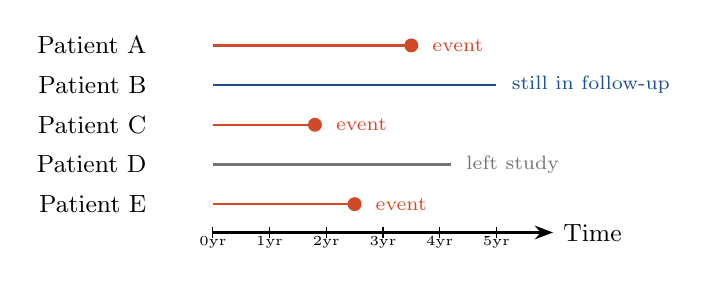
\begin{tikzpicture}[>=Stealth,scale=0.72]
    \node[left,font=\small] at (0,2.8) {Patient A};
    \draw[thick,columbiaaccent] (1,2.8) -- (4.5,2.8);
    \fill[columbiaaccent] (4.5,2.8) circle (3.5pt);
    \node[right,font=\scriptsize,columbiaaccent] at (4.7,2.8) {event};

    \node[left,font=\small] at (0,2.1) {Patient B};
    \draw[thick,columbia] (1,2.1) -- (6.0,2.1);
    \node[right,font=\scriptsize,columbia] at (6.1,2.1) {still in follow-up};

    \node[left,font=\small] at (0,1.4) {Patient C};
    \draw[thick,columbiaaccent] (1,1.4) -- (2.8,1.4);
    \fill[columbiaaccent] (2.8,1.4) circle (3.5pt);
    \node[right,font=\scriptsize,columbiaaccent] at (3.0,1.4) {event};

    \node[left,font=\small] at (0,0.7) {Patient D};
    \draw[thick,columbiagray] (1,0.7) -- (5.2,0.7);
    \node[right,font=\scriptsize,columbiagray] at (5.3,0.7) {left study};

    \node[left,font=\small] at (0,0) {Patient E};
    \draw[thick,columbiaaccent] (1,0) -- (3.5,0);
    \fill[columbiaaccent] (3.5,0) circle (3.5pt);
    \node[right,font=\scriptsize,columbiaaccent] at (3.7,0) {event};

    \draw[->,thick] (1,-0.5) -- (7,-0.5) node[right,font=\small] {Time};
    \foreach \x in {0,1,...,5} {
        \draw (1+\x,-0.6) -- (1+\x,-0.4) node[below,font=\tiny] {\x yr};
    }
\end{tikzpicture}
\end{center}

\vspace{-0.3em}
{\small B and D are \textbf{right-censored}: survived at least this long, true event time unknown. Dropping them wastes data; treating them as events is wrong.}

\vspace{0.05em}
{\scriptsize \textbf{Key assumption:} Censoring is \emph{non-informative}---patients who drop out aren't systematically sicker or healthier. If they are, estimates are biased.}

\vspace{0.05em}
{\scriptsize \textbf{Competing risks:} Patient D might have died of something unrelated---making the event of interest impossible, not just unobserved.}
\end{frame}

% --- Point 9: clarify S(t) population/patient, simplify h(t) ---
\begin{frame}{Survival Concepts --- Before Any Model}
\textbf{Two quantities we want to estimate:}

\vspace{0.2em}
\textbf{Survival function:} \; $S(t) = P(T > t)$

{\small The probability that a patient drawn from this population survives past time $t$. For an individual, we interpret it probabilistically: ``given what we know, what's the chance this patient is still event-free at time $t$?'' Starts at 1, decreases.}

\vspace{0.2em}
\textbf{Hazard function:} The instantaneous event rate among those who haven't had the event yet---``given that you've survived this long, how quickly are events happening \emph{right now}?''

\vspace{0.1em}
{\small Formally: $h(t) = -\dfrac{d}{dt}\ln S(t)$}

\vspace{0.2em}
\pause
These are mathematically linked: knowing one determines the other. \textbf{Kaplan-Meier} estimates $S(t)$. \textbf{Cox PH} models $h(t)$ as a function of covariates.
\end{frame}

% --- Point 10: simple KM intro before formula ---
\begin{frame}{Kaplan-Meier Estimator}
\textbf{The intuition:} At any time $t$, count how many patients are still being followed who haven't had the event. Each time someone has the event, the estimated survival probability steps down. Censored patients leave the count quietly---without causing a step.

\vspace{0.2em}
\pause
\textbf{Formally:} At each event time $t_j$,
\[
    \hat{S}(t) = \prod_{t_j \leq t} \left(1 - \frac{d_j}{n_j}\right)
\]
where $d_j$ = events at $t_j$, \; $n_j$ = patients still at risk (haven't had the event and haven't been censored yet).

\vspace{0.1em}
$\hat{S}(t)$ is a \textbf{step function}: it drops at each event time and stays flat in between. \textbf{Log-rank test:} compares two K-M curves ($H_0$: no difference).
\end{frame}

% ============================================================
\begin{frame}{Reading a Kaplan-Meier Curve}
\begin{center}
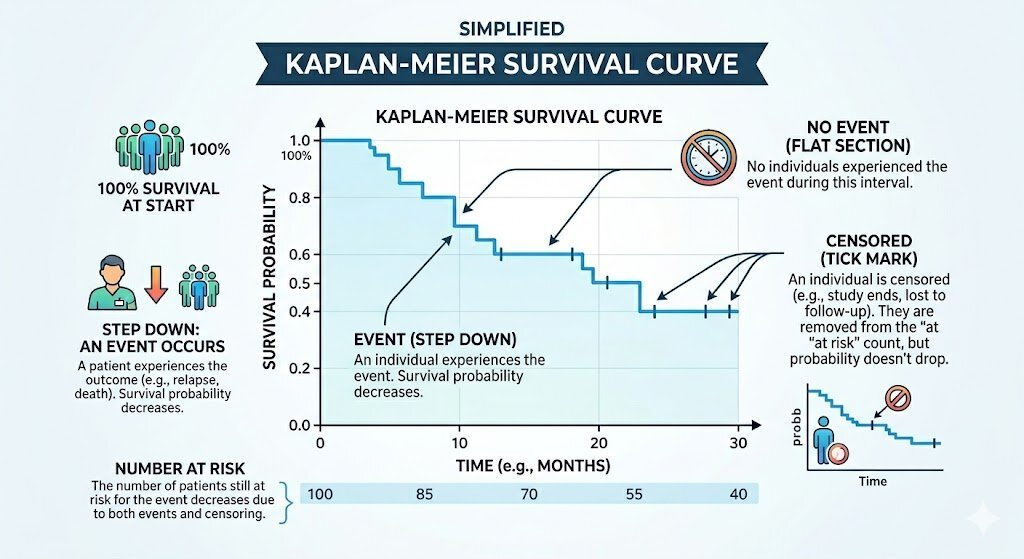
\includegraphics[width=\textwidth,height=0.82\textheight,keepaspectratio]{km_explainer.jpg}
\end{center}
\end{frame}

% --- Point 11: fix worked example column headers, clarify S(t) at each time ---
\begin{frame}{Kaplan-Meier: A Worked Example}
\textbf{Five patients from the censoring diagram.} $\hat{S}$ starts at 1 and updates at each event:

\vspace{0.2em}
\begin{center}
{\small
\renewcommand{\arraystretch}{1.15}
\begin{tabular}{cccccc}
\toprule
\textbf{Time} & \textbf{What happened} & $d_j$ & $n_j$ & $1 - d_j/n_j$ & $\hat{S}$ \textbf{after} \\
\midrule
0--1.8 yr & (no events yet) & & & & 1.000 \\
1.8 yr & \textcolor{columbiaaccent}{Event (C)} & 1 & 5 & 4/5 & $1 \times \tfrac{4}{5} = 0.800$ \\
2.5 yr & \textcolor{columbiaaccent}{Event (E)} & 1 & 4 & 3/4 & $0.8 \times \tfrac{3}{4} = 0.600$ \\
3.5 yr & \textcolor{columbiaaccent}{Event (A)} & 1 & 3 & 2/3 & $0.6 \times \tfrac{2}{3} = 0.400$ \\
4.2 yr & \textcolor{columbiagray}{Left study (D)} & --- & \multicolumn{3}{l}{$n$ drops from 2 to 1; $\hat{S}$ unchanged} \\
5.0+ yr & \textcolor{columbia}{Still followed (B)} & --- & \multicolumn{3}{l}{$n = 1$; no more events observed} \\
\bottomrule
\end{tabular}
}
\end{center}

\vspace{0.1em}
Between events, $\hat{S}$ is \emph{constant}. E.g., $\hat{S}(2.0) = \hat{S}(2.4) = 0.800$.
\end{frame}

% ============================================================
\begin{frame}{K-M on Real Data: Population and Subgroups}
\begin{center}
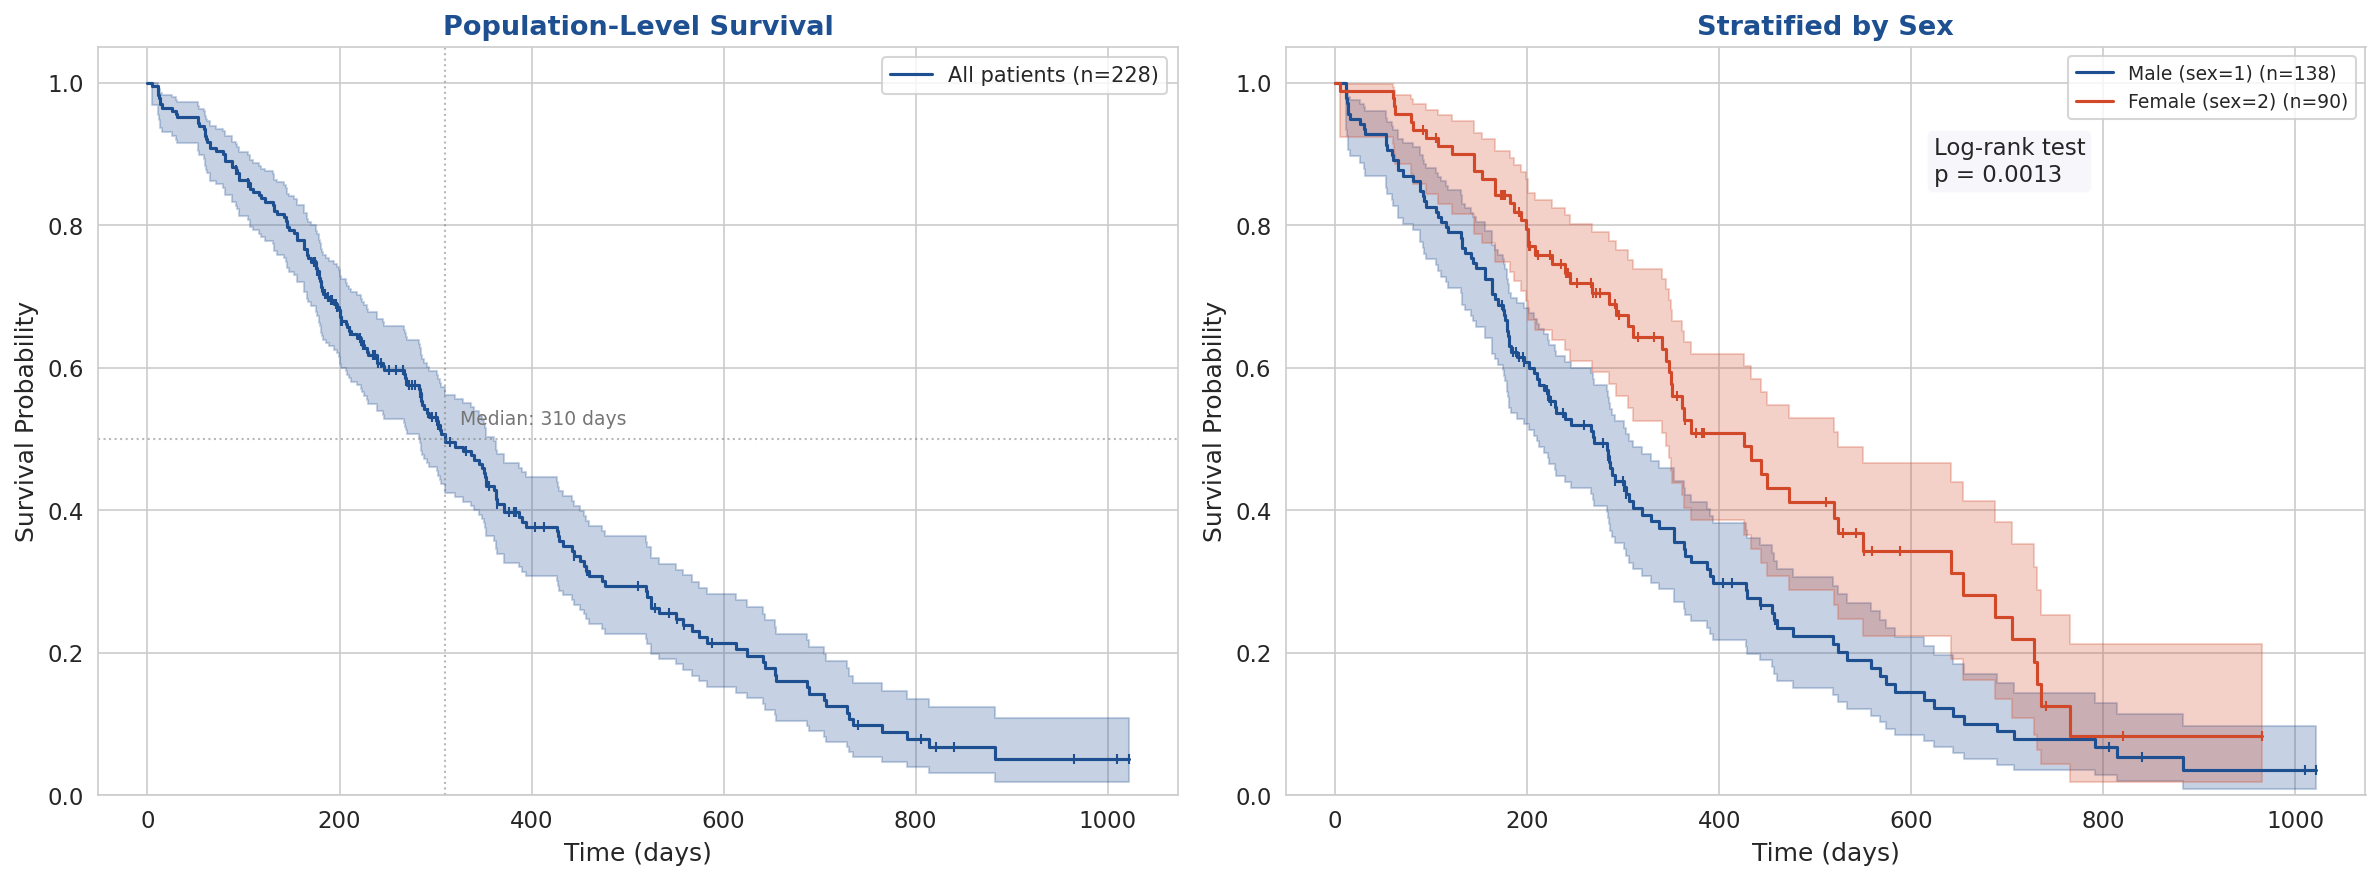
\includegraphics[width=\textwidth,height=0.62\textheight,keepaspectratio]{fig3_kaplan_meier.png}
\end{center}
\vspace{-0.3em}
{\scriptsize NCCTG Lung Cancer dataset (lifelines). Left: population-level K-M curve with median survival. Right: stratified by sex---subgroup differences emerge. The point is how to \emph{read} K-M curves: step functions, censoring marks ($|$), confidence bands, log-rank comparison.}
\end{frame}

% ============================================================
\begin{frame}{Cox Proportional Hazards}
\textbf{Model the hazard as a function of covariates:}
\[
    h(t \mid X) = h_0(t) \cdot \exp(\beta_1 X_1 + \cdots + \beta_p X_p)
\]

\begin{itemize}
    \item $h_0(t)$: baseline hazard (left unspecified---\textbf{semi-parametric})
    \item $\exp(\beta_j)$: \textbf{hazard ratio} for covariate $j$. \; HR $> 1$: higher risk. HR $< 1$: protective.
    \item \textbf{PH assumption:} the ratio of hazards between any two patients is constant over time
\end{itemize}

\vspace{0.1em}
\pause
\alert{Are these hazard ratios causal?} Only if confounders are controlled. From a registry: \textbf{associational}. From an RCT: \textbf{causal}. The data source determines the interpretation, not the model.
\end{frame}

% ============================================================
\begin{frame}{Cox PH on Real Data (Notebook Fig.~4)}
\begin{center}
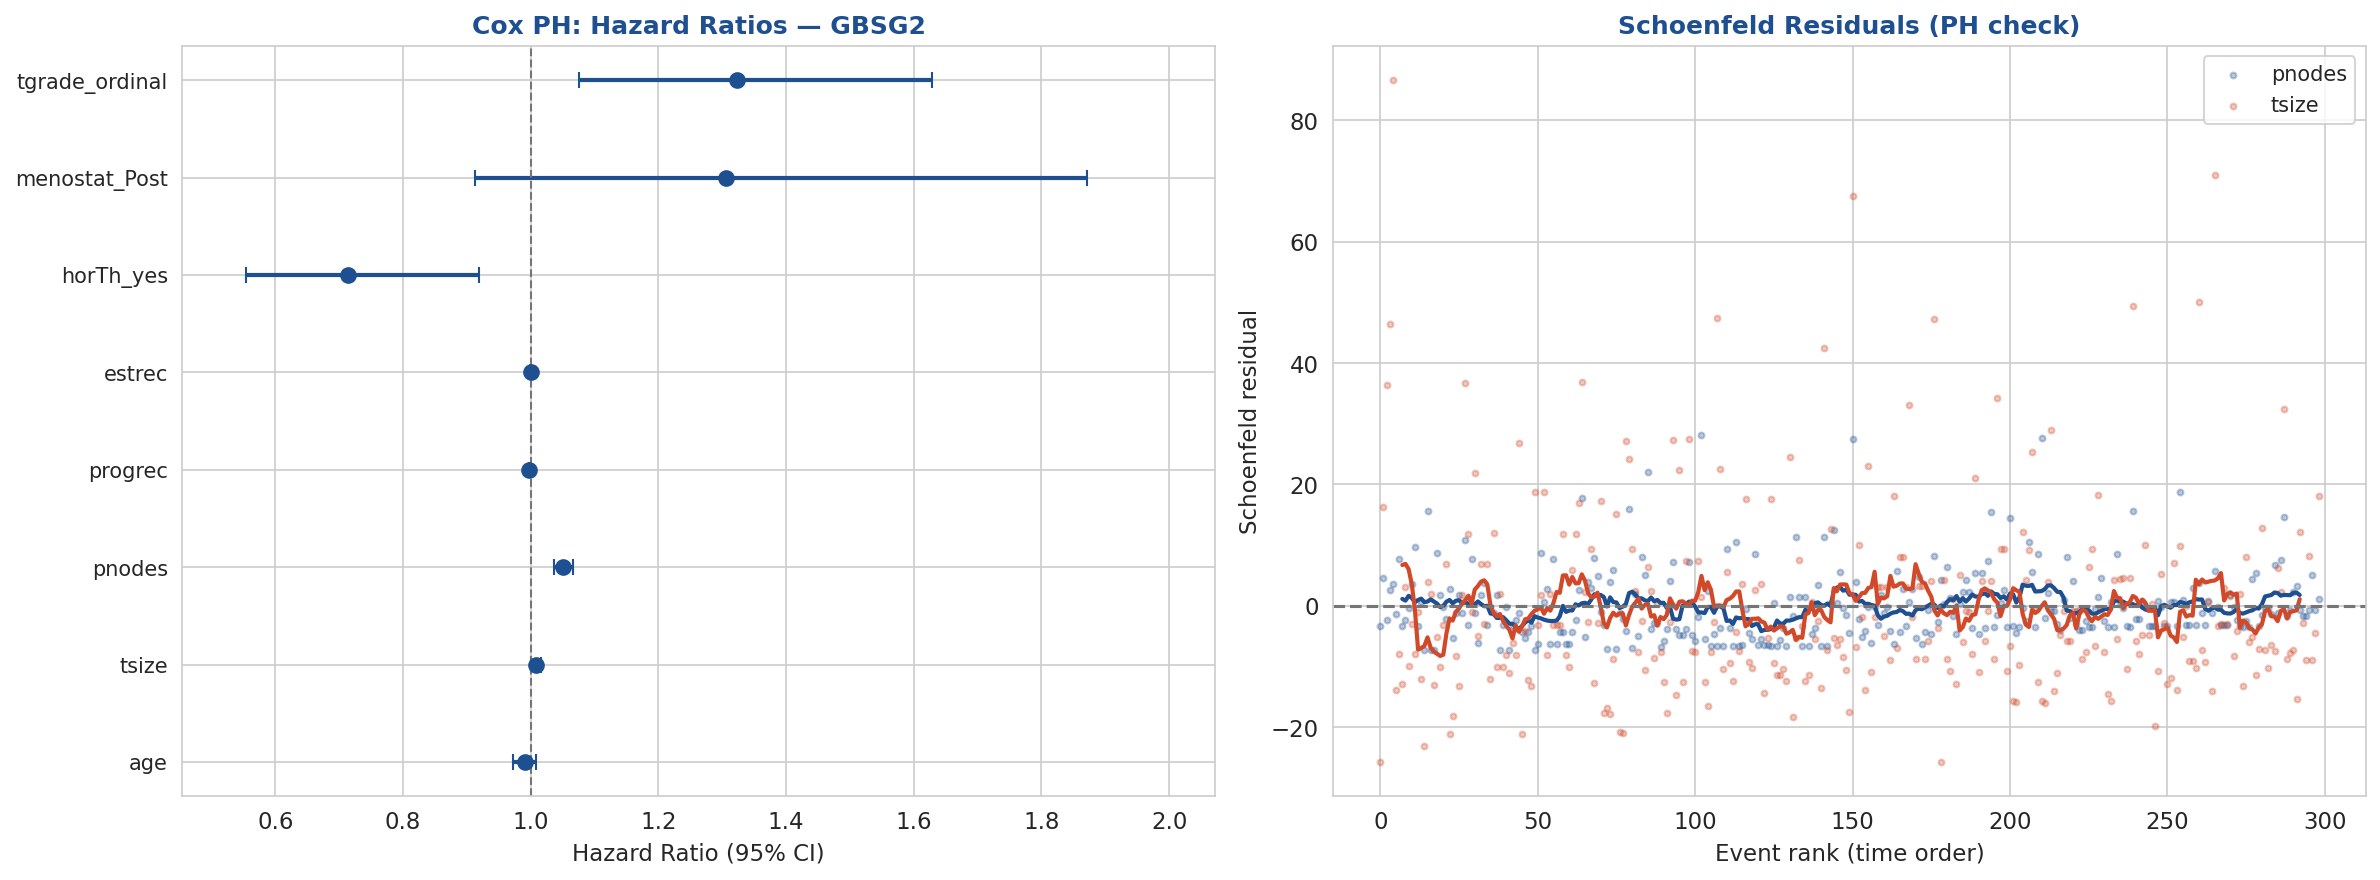
\includegraphics[width=\textwidth,height=0.60\textheight,keepaspectratio]{fig4_cox_forest.png}
\end{center}
\vspace{-0.3em}
{\scriptsize GBSG2 breast cancer RCT (lifelines, 686 patients). Left: hazard ratios with 95\% CI (features ordered by effect size). Right: \textbf{Schoenfeld residuals}---a diagnostic for the PH assumption. Each covariate gets a residual at each event time; if PH holds, these should show no trend. A slope means the covariate's effect \emph{changes} over time (e.g., a drug that works initially but wears off). Flat-looking patterns are consistent with PH for that covariate.}
\end{frame}

% --- Point 12: mention DeepSurv and beyond in main deck ---
\begin{frame}{Beyond Cox: Modern Survival Models}
Cox PH assumes the log-hazard is a \emph{linear} function of covariates. What if it isn't?

\vspace{0.2em}
\textbf{DeepSurv} (Katzman et al., 2018): replace $\beta^\top X$ with a neural network $f_\theta(X)$, keep the same loss function (partial likelihood). Helps when there are non-linear interactions and large $n$.

\vspace{0.2em}
\textbf{Other approaches:}
\begin{itemize}
    \item \textbf{Random survival forests:} ensemble methods for survival data
    \item \textbf{Discrete-time models:} bin time, use standard classifiers per bin
    \item \textbf{DeepHit} (Lee et al., 2018): directly estimate the probability of events in each time bin
\end{itemize}

\vspace{0.2em}
\pause
{\small \textbf{Caveat:} On small tabular datasets (like GBSG2), Cox often matches or beats neural approaches. Depth helps most with high-dimensional inputs (imaging, genomics) and large $n$. See notebook appendix for a DeepSurv vs.\ Cox comparison.}
\end{frame}

% ============================================================
\section{Synthesis}
% ============================================================

\begin{frame}{Back to Our Question}
\textbf{Which kidney stone treatment is better?}

\vspace{0.2em}
\pause
\begin{enumerate}[<+->]
    \item \textbf{EHR:} One hospital, small $n$, severity not captured, treatment chosen by clinician. Insufficient alone for a causal answer.
    \item \textbf{Registry:} Better coverage---but Simpson's Paradox shows confounding by stone size reverses the comparison.
    \item \textbf{RCT:} Randomization balances confounders in expectation---but expensive, narrow population, possibly unethical for surgical comparisons.
    \item \textbf{In practice:} Combine evidence sources. Interpret results in light of the data source. Meta-analyses synthesize across studies.
\end{enumerate}

\onslide<5->{\vspace{0.1em}
\textbf{Thursday (L24):} Causal inference methods that let us extract stronger answers from observational data---and what happens when the \emph{outcome you're measuring} is itself biased.}
\end{frame}

% --- Point 13: stronger summary ---
\begin{frame}{Summary}
\textbf{Part I: Population Health Data}
\begin{itemize}
    \item The question you're asking determines the data you need: descriptive, predictive, or causal.
    \item EHR data is convenient but confounded. Registries improve coverage but don't eliminate confounding (Simpson's Paradox). RCTs address confounding by randomization but are expensive and narrow.
    \item Biobanks blur the designed/byproduct boundary. Volunteer-based cohorts are especially vulnerable to healthy volunteer bias.
    \item Causal inference methods can strengthen observational analyses---and reveal when outcomes themselves are biased. Thursday's topic.
\end{itemize}

\vspace{0.2em}
\textbf{Part II: Survival Analysis}
\begin{itemize}
    \item Time-to-event outcomes require handling censoring and competing risks.
    \item K-M estimates population survival; Cox PH models hazard as a function of covariates.
    \item Whether hazard ratios are causal depends on the data source, not the model.
\end{itemize}
\end{frame}

% ============================================================
\begin{frame}[standout]
    Questions?
\end{frame}

% ============================================================
\appendix
% ============================================================

\begin{frame}{Appendix: How Cox Is Fit --- The Partial Likelihood}
\textbf{Key insight:} We never estimate $h_0(t)$. At each event, we ask: among those still at risk, did the right one die?

\[
    L(\beta) = \prod_{i:\,\delta_i=1} \frac{\exp(\beta^\top X_i)}{\displaystyle\sum_{j \in \mathcal{R}(t_i)} \exp(\beta^\top X_j)}
\]

Each term is a \textbf{softmax} over the risk set. Only ranking matters---the concordance index ($C$-index) is a standard evaluation metric. DeepSurv uses exactly this loss with $f_\theta(X)$ replacing $\beta^\top X$.
\end{frame}

\begin{frame}{Appendix: DeepSurv vs.\ Cox (Notebook Fig.~5)}
\begin{center}
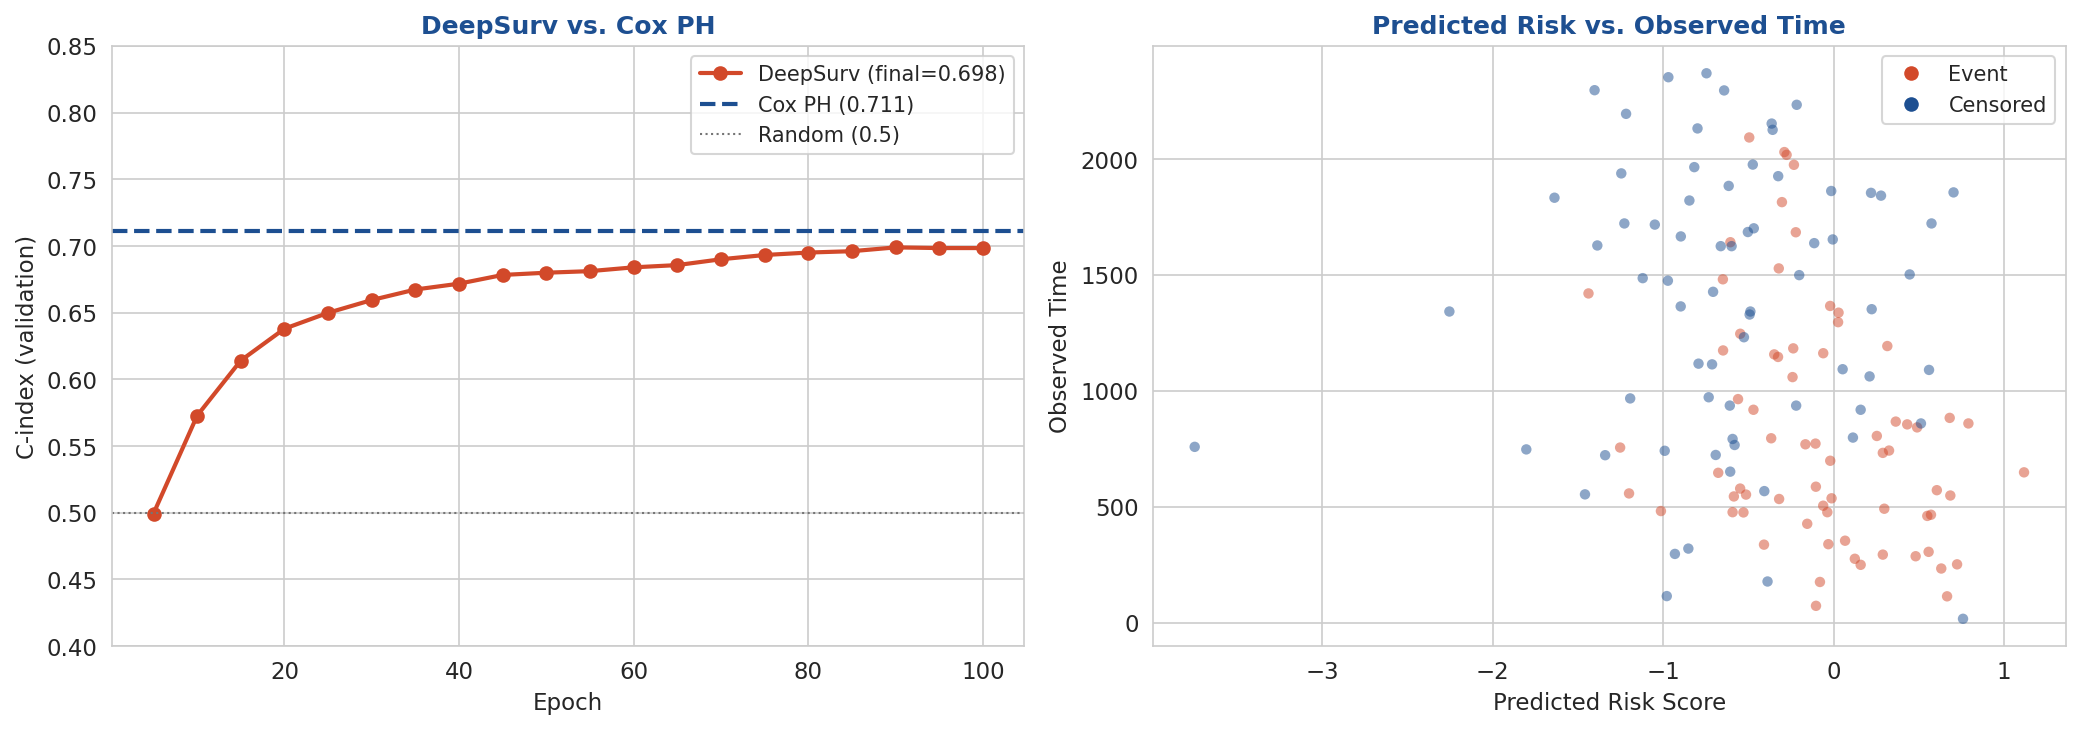
\includegraphics[width=\textwidth,height=0.65\textheight,keepaspectratio]{fig5_deepsurv_comparison.png}
\end{center}
\vspace{-0.3em}
{\scriptsize GBSG2: DeepSurv (C=0.698) slightly underperforms Cox (C=0.711). Expected on small tabular data with few covariates. Single-seed demo.}
\end{frame}

\begin{frame}{Appendix: Propensity Scores (Preview for L24)}
\textbf{Propensity score} $e(X) = P(\text{Treatment} = 1 \mid X)$. Match or reweight patients to approximate randomization from observational data. Only adjusts for \emph{measured} confounders.

\begin{center}
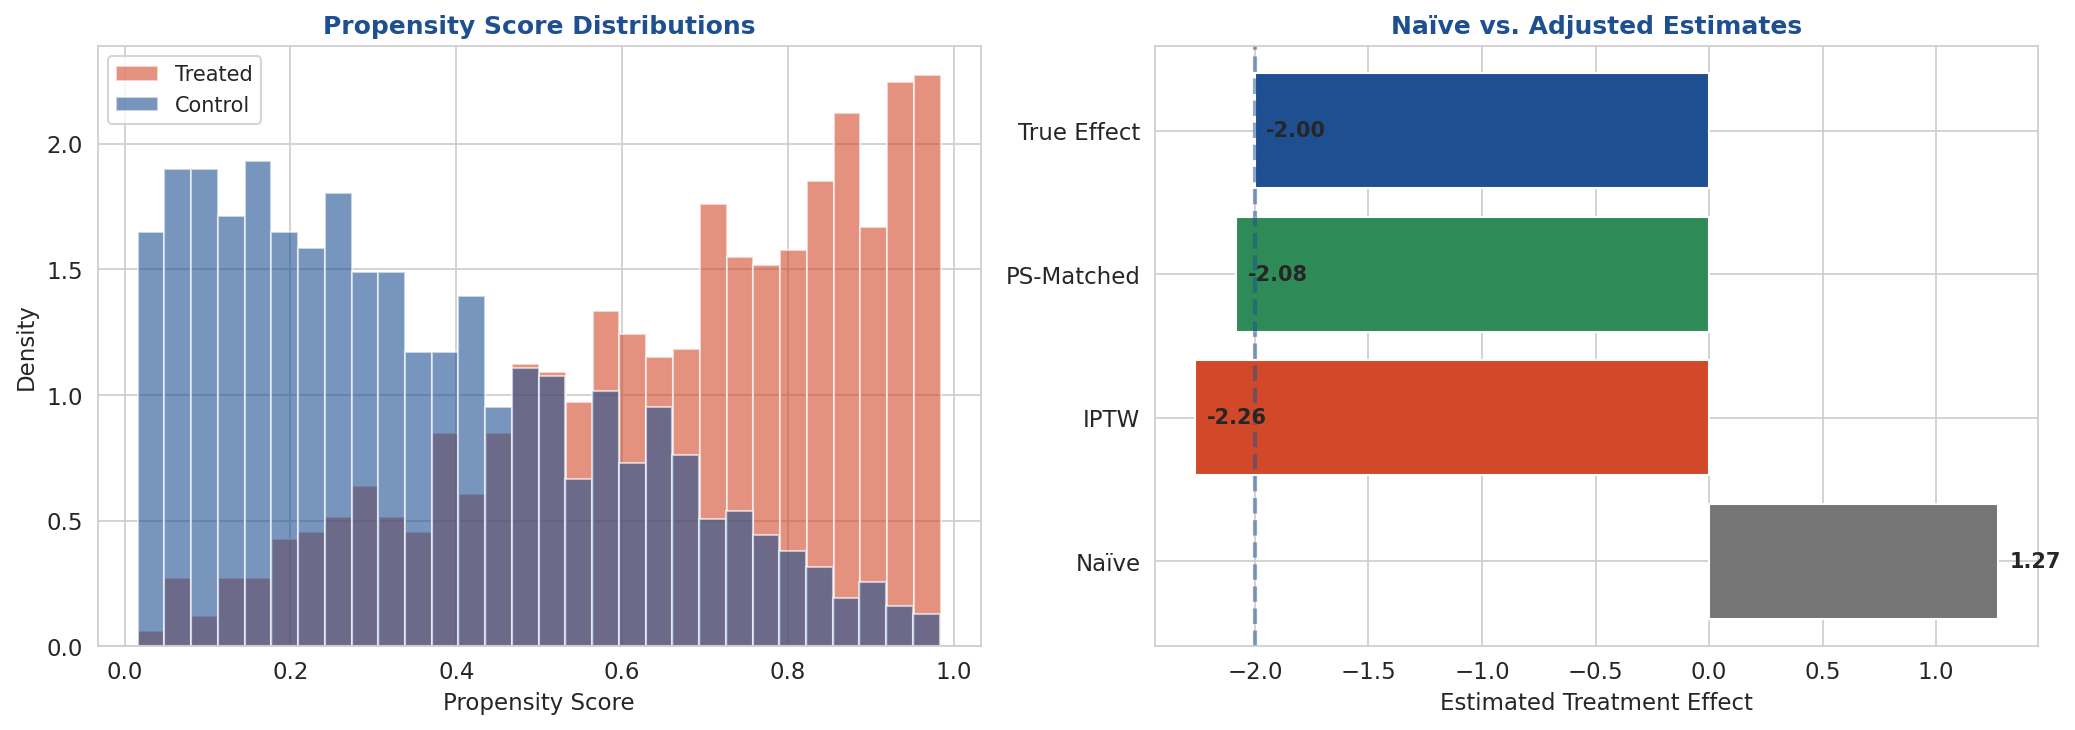
\includegraphics[width=0.85\textwidth,height=0.42\textheight,keepaspectratio]{fig6_propensity_scores.png}
\end{center}
\vspace{-0.3em}
{\scriptsize Simulated data with known true effect. Na\"ive estimate is biased; PS adjustment recovers closer to truth. Full treatment Thursday (L24).}
\end{frame}

\begin{frame}{Appendix: References}
\tiny
\begin{columns}[T]
\column{0.48\textwidth}
\textbf{Simpson's Paradox:}\\
Charig et al.\ (1986). Renal calculi treatment. \textit{BMJ}.\\[0.1em]

\textbf{Registries \& population data:}\\
SEER: \texttt{seer.cancer.gov}\\
NHANES: \texttt{wwwn.cdc.gov/nchs/nhanes}\\
Fry et al.\ (2017). UK Biobank vs.\ general population. \textit{Am J Epi}.\\
Batty et al.\ (2020). Risk factor associations in UK Biobank vs.\ representative cohorts.\\
Murthy et al.\ (2004). Trial participants vs.\ cancer population.\\
Travers et al.\ (2007). External validity of asthma RCTs. \textit{Thorax}.\\[0.1em]

\textbf{Survival analysis:}\\
Cox (1972). Regression models and life-tables. \textit{JRSS-B}.\\
Kaplan \& Meier (1958). Nonparametric estimation. \textit{JASA}.\\

\column{0.48\textwidth}
\textbf{Modern survival models:}\\
Katzman et al.\ (2018). DeepSurv. \textit{BMC Med Res Meth}.\\
Lee et al.\ (2018). DeepHit.\\
Ishwaran et al.\ (2008). Random survival forests. \textit{Ann Appl Stat}.\\[0.1em]

\textbf{Propensity scores:}\\
Rosenbaum \& Rubin (1983). Propensity score. \textit{Biometrika}.\\[0.1em]

\textbf{Clinical trials:}\\
ClinicalTrials.gov: \texttt{clinicaltrials.gov/api}\\[0.1em]

\textbf{Biobanks:}\\
\texttt{ukbiobank.ac.uk}\\
\texttt{allofus.nih.gov}\\
\texttt{biobankjp.org}
\end{columns}
\end{frame}

\begin{frame}{Appendix: Trial Phases \& Costs}
{\small
\begin{center}
\renewcommand{\arraystretch}{1.15}
\begin{tabular}{lrrp{4.5cm}}
\toprule
\textbf{Phase} & \textbf{Typical $n$} & \textbf{Duration} & \textbf{Goal} \\
\midrule
Phase I & 20--80 & months & Safety, dosing \\
Phase II & 100--300 & 1--2 years & Efficacy signal \\
Phase III & 1K--10K & 2--4 years & Definitive efficacy \\
Phase IV & 10K+ & ongoing & Post-market surveillance \\
\bottomrule
\end{tabular}
\end{center}
}
\end{frame}

\begin{frame}{Appendix: CDISC/SDTM Data Standards}
\textbf{CDISC} standardizes trial data for FDA submission: Demographics (DM), Adverse Events (AE), Labs (LB), Vital Signs (VS). Each domain is a flat table with standardized variable names.

\vspace{0.2em}
\textbf{Analogy:} DICOM for imaging (L21), ICD/LOINC for EHR codes (L17), CDISC for trials.
\end{frame}

\end{document}
